\documentclass[tikz,border=8pt]{standalone}
% Shared look for every TikZ diagram. Load with \input{../../tools/tikz-style.tex}
\usepackage[T1]{fontenc}
\usepackage{lmodern}
\renewcommand{\sfdefault}{lmr}  % diagrams use the same serif as the text
\usetikzlibrary{arrows.meta, positioning, shapes.geometric, calc, fit, backgrounds}
\definecolor{cblue}{HTML}{4C78A8}
\definecolor{corange}{HTML}{F58518}
\definecolor{cgreen}{HTML}{54A24B}
\definecolor{cred}{HTML}{E45756}
\definecolor{cpurple}{HTML}{B279A2}
\definecolor{cgrey}{HTML}{6B6B6B}
\tikzset{
  every picture/.style={font=\sffamily, line width=1.2pt},
  box/.style={draw=#1, fill=#1!12, rounded corners=4pt, align=center, inner sep=7pt, minimum height=1.1cm},
  box/.default=cgrey,
  arrow/.style={-{Stealth[length=3mm]}, draw=cgrey, line width=1.4pt},
  title/.style={font=\sffamily\bfseries\Large},
  note/.style={font=\sffamily\small, text=cgrey, align=center},
}
\AtBeginDocument{\hyphenpenalty=10000 \exhyphenpenalty=10000}

\begin{document}
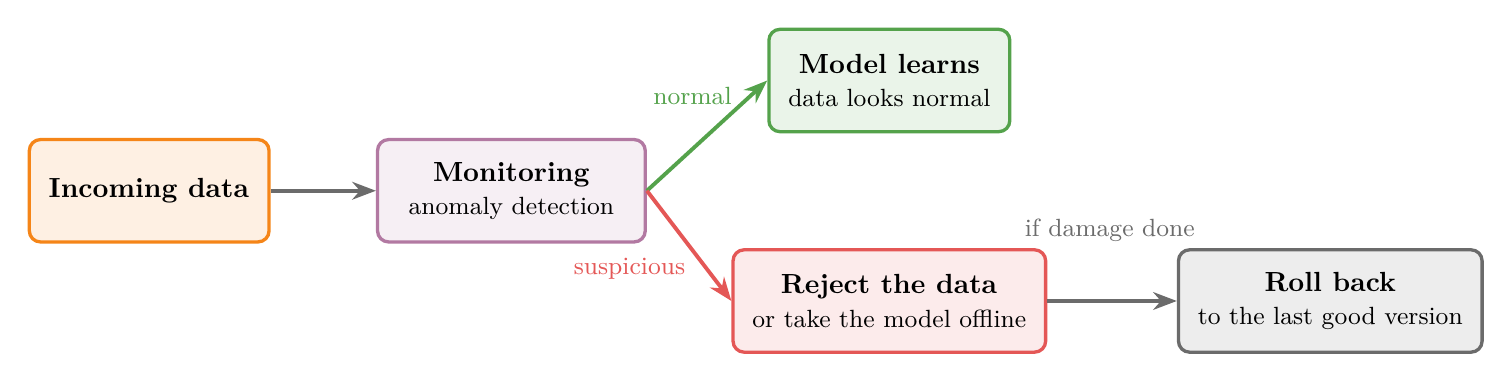
\begin{tikzpicture}
  \node[box=corange, minimum width=2.8cm, minimum height=1.3cm] (in) at (0,0) {\textbf{Incoming data}};
  \node[box=cpurple, minimum width=3.4cm, minimum height=1.3cm] (mon) at (4.6,0) {\textbf{Monitoring}\\{\small anomaly detection}};
  \node[box=cgreen, minimum width=3.0cm, minimum height=1.3cm] (learn) at (9.4,1.4) {\textbf{Model learns}\\{\small data looks normal}};
  \node[box=cred, minimum width=3.0cm, minimum height=1.3cm] (rej) at (9.4,-1.4) {\textbf{Reject the data}\\{\small or take the model offline}};
  \node[box=cgrey, minimum width=3.4cm, minimum height=1.3cm] (back) at (15.0,-1.4) {\textbf{Roll back}\\{\small to the last good version}};
  \draw[arrow] (in) -- (mon);
  \draw[arrow, draw=cgreen] (mon.east) -- (learn.west);
  \node[note, text=cgreen] at (6.9,1.2) {normal};
  \draw[arrow, draw=cred] (mon.east) -- (rej.west);
  \node[note, text=cred] at (6.1,-1.0) {suspicious};
  \draw[arrow] (rej) -- (back);
  \node[note] at (12.2,-0.5) {if damage done};
\end{tikzpicture}
\end{document}
